\chapter{Data}

\section{Datasets}

\subsection{Lyrics dataset}
 We chose the \textit{55000+ Song Lyrics dataset} from
 Kaggle.com\footnote{https://www.kaggle.com/mousehead/songlyrics} to obtain lyrics
 data. The Kaggle dataset originally contained 57 650 English songs. It’s lyrics are
 scraped from LyricsFreak\footnote{https://www.lyricsfreak.com}. Extremely long and short lyrics were removed as well as
 all non-ASCII symbols from the lyrics. Figure \ref{fig:lyrics_dataset} shows the
 first two entries of the dataset.\\
 \begin{figure}[h]
    \centering
	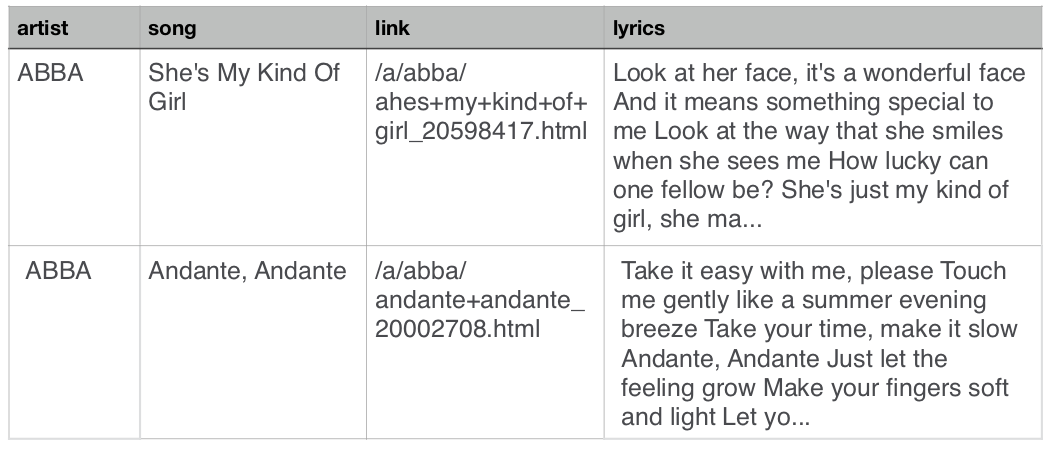
\includegraphics[height=60mm]{./img/dataset_preview.png}
	\caption{First two entries of the 55000+ Lyrics Dataset}
	\label{fig:lyrics_dataset}
\end{figure}

\subsection{User-information dataset}
To evaluate text and audio based methods on real-life user data, we had to select a
dataset containing song information and lyrics as well as a dataset with information
about users and their played tracks. First we tried to match the lyrics dataset onto
the \textit{Thisismyjam} dataset\footnote{http://www.thisismyjam.com}. However we
were able to match only 6800 songs with lyrics as well as user data. We then tried
the \textit{Echo Nest Subset profile}\footnote{https://labrosa.ee.columbia.edu/millionsong/tasteprofile} \cite{Bertin-Mahieux2011} dataset available
on the Milion Song Dataset (=MSD) website. 
The Echo Nest Taste Profile Subset provides us with 48,373,586 triplets of
\textit{user id, song id} and \textit{the number of times the user has played a
song}. This then had to be mapped onto the MSD dataset to get a name and artist for each song and then onto our lyrics dataset.

After removing songs we did not have lyrics for, we ended up with 16,594 unique songs, and 45,054 unique users. Even though it is a significant reduction it still provides enough data to carry out all the desired experiments. For each of the 16,594 songs we also acquired a mono .wav
file. 

\section{Final dataset statistics}
Overall our final dataset had 160,454 entries containing a user id, artist, song title and lyrics. We extracted two of different datasets suited for different tasks throughout the thesis.
\begin{itemize}
    \item The \textit{Song dataset} denoted as SD in this work. It contains the
    16,594 unique songs with their metadata (title, artist, lyrics and audio), the users were omitted.
    \item The \textit{User dataset} denoted as UD. It contains 11,123 unique users who have at least 4 songs in their playlist. Each one of 110,826 entries consists of a userID, song name and artist. 
\end{itemize}
 Since the evaluation method is aimed to reveal the missing entries based on the
 implemented recommendation techniques\footnote{Chapter \ref{chap:experiments}} we studied the dataset and especially the playlist's
 lengths in more detail.
 
Here are some important remarks:
\begin{itemize}
    \item Each user only has one playlist. This means there is a one to one mapping between users and playlists and the terms are used interchangeably.
    \item We do not know which songs the user has played most recently.
    \item Users with only one song are useless for the purpose of evaluation.
\end{itemize} 
When analyzing our dataset, it turned out, that out of 45,054 playlists, there are 22,257 with only one song, which leaves us with 22,797 we can use. We however decided to use only playlists of length at least four for evaluation because it still leaves us with enough unique playlists --- 11,123 to be specific --- and allows us to study deeper connections than song to song similarities. 

The distribution of the lengths for useful playlists is shown in more detail in Figure
\ref{fig:playlist_length_distribution}. We can see that most of the playlists are
short, almost a third of them only contains two songs. The average number of songs
per playlists (including those containing only one song) is 3.56. 
\begin{figure}[]
    \centering
	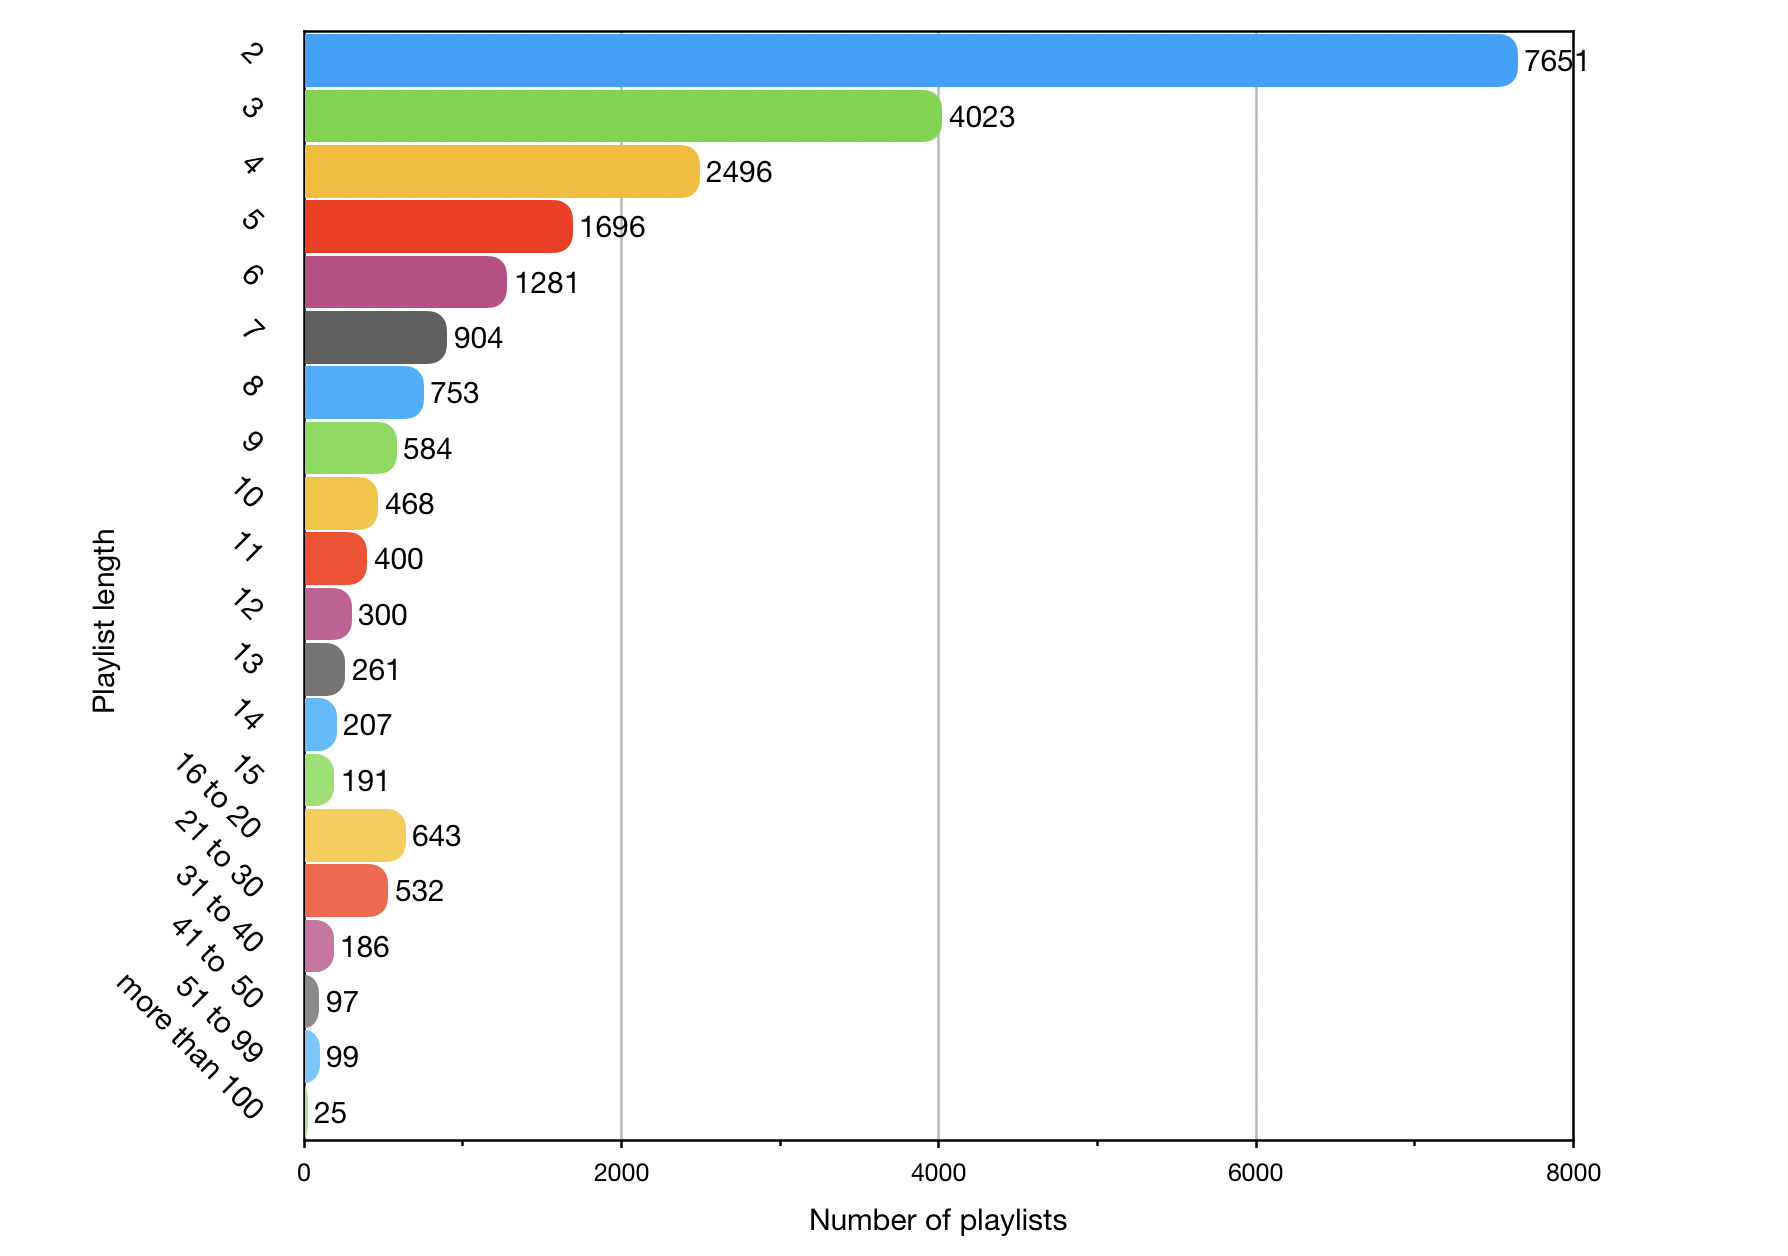
\includegraphics[width=1\linewidth]{./img/playlist_length_numbers.png}
	\caption{Playlists' lengths histogram}
	\label{fig:playlist_length_distribution}
\end{figure}

The average number of playlists a song from our dataset belongs to is 10.84. The
distribution and the most popular songs are depicted in Figure
\ref{fig:popular_song_distribution}. The by far most popular song with a total of 816
plays was \textit{Royals} by \textit{Lorde}. Second came \textit{Radioactive} by
\textit{Imagine Dragons} with 674 users who played it. All other songs have been
played by less than 500 users.

\begin{figure}[]
    \centering
	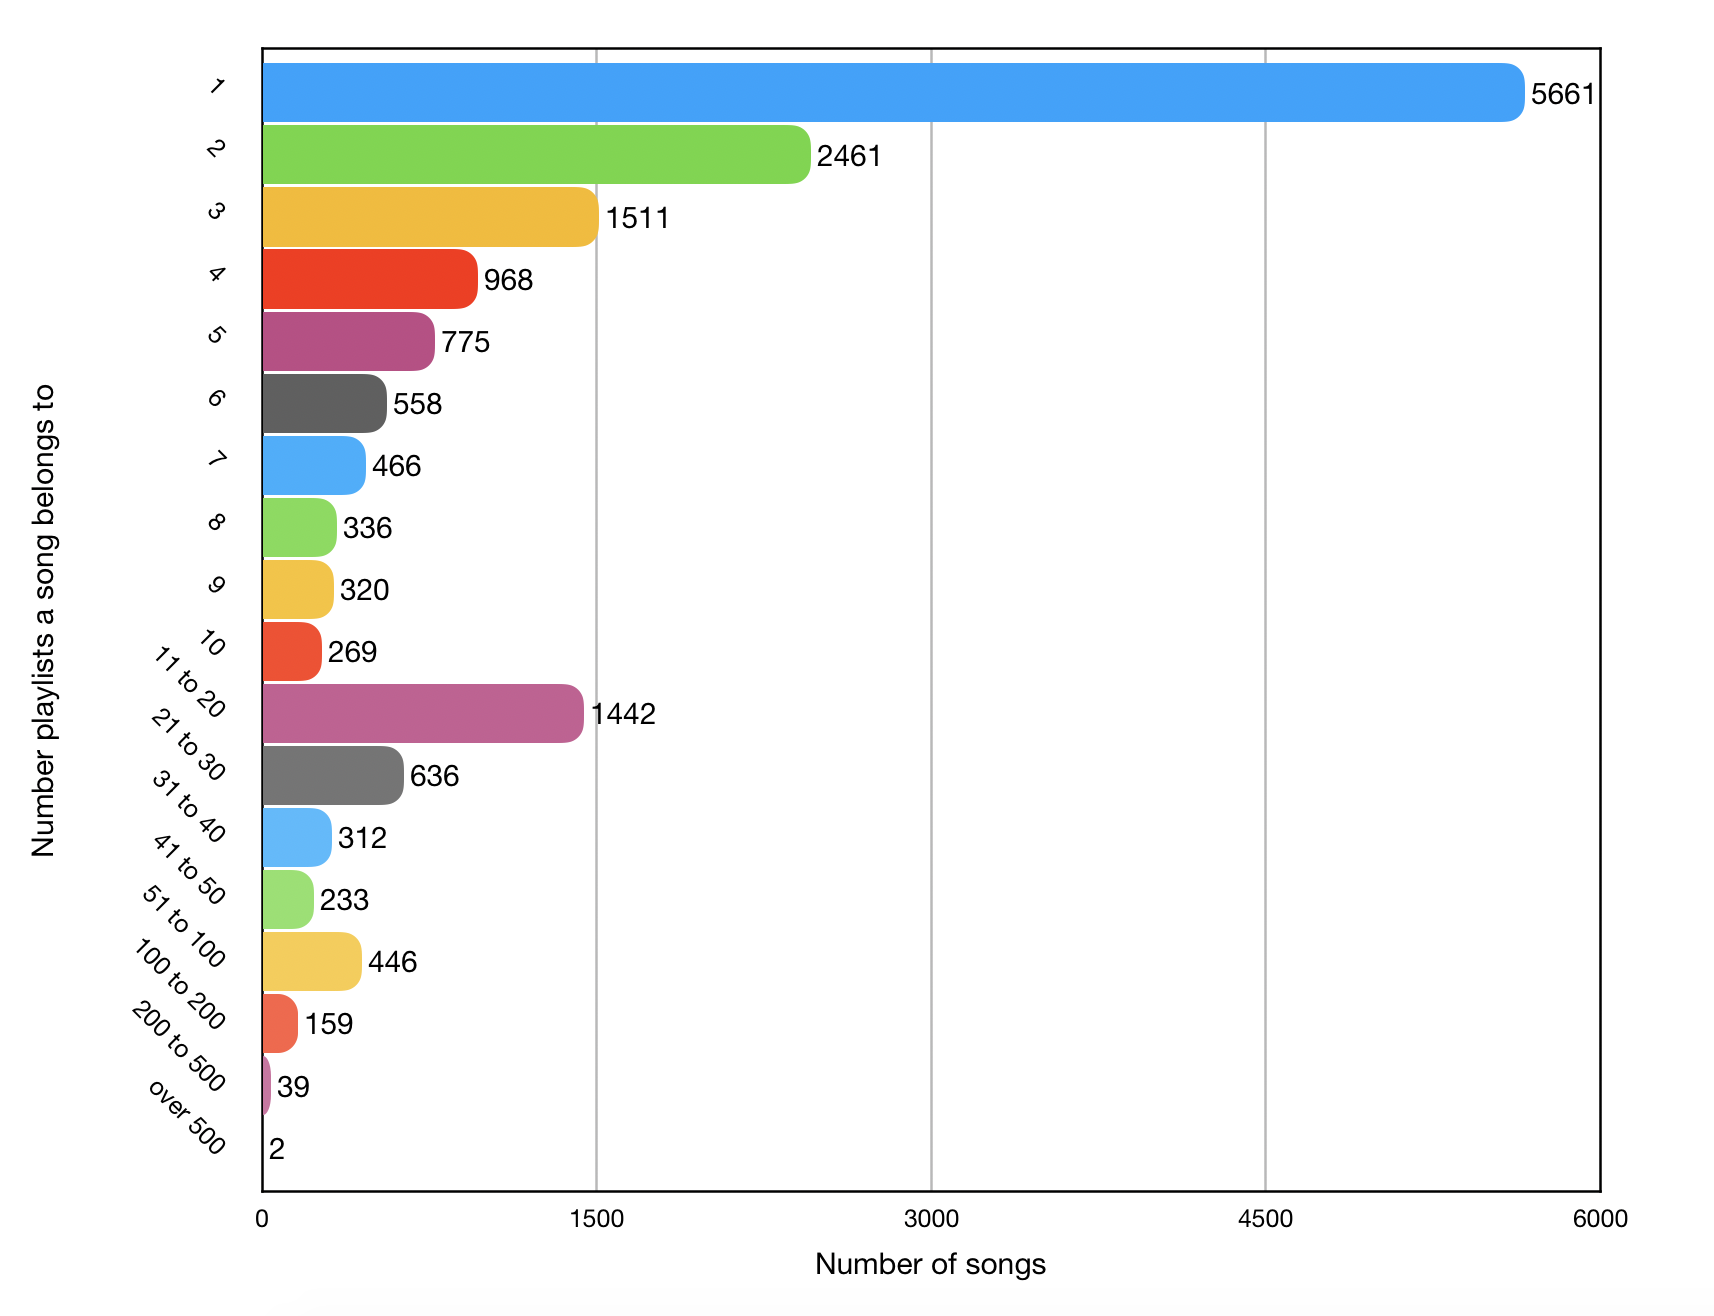
\includegraphics[width=1\linewidth]{./img/times_played_numbers2.png}
	\caption{The histogram of playlist counts per individual songs}
	\label{fig:popular_song_distribution}
\end{figure}
